\documentclass[aspectratio=169,12pt,t]{beamer}

% --- Theme: Metropolis (modern, clean) ---
\usetheme[progressbar=frametitle,numbering=fraction,block=fill]{metropolis}

% --- Fira Sans font (install texlive-fonts-extra if missing) ---
\IfFileExists{FiraSans.sty}{\usepackage[sfdefault]{FiraSans}}{}

% --- Light background with warm accent ---
\definecolor{mDarkTeal}{RGB}{35,55,59}
\definecolor{mLightBrown}{RGB}{235,228,216}
\definecolor{mAccent}{RGB}{140,70,20}

\setbeamercolor{normal text}{fg=mDarkTeal,bg=white}
\setbeamercolor{alerted text}{fg=mAccent}
\setbeamercolor{frametitle}{bg=mDarkTeal,fg=white}
\setbeamercolor{progress bar}{fg=mAccent,bg=mLightBrown}
\setbeamercolor{title separator}{fg=mAccent}
\setbeamercolor{progress bar in head/foot}{fg=mAccent,bg=mLightBrown}
\setbeamercolor{progress bar in section page}{fg=mAccent,bg=mLightBrown}

% --- Packages ---
\usepackage[utf8]{inputenc}
\usepackage{amsmath,amssymb,amsthm}
\usepackage{mathrsfs}
\usepackage{tikz}
\usetikzlibrary{arrows.meta,positioning,calc,decorations.pathreplacing,shapes,patterns}
\usepackage{pgfplots}
\pgfplotsset{compat=1.18}

% --- Semi-transparent white highlight for text on top of background images ---
\usepackage[most]{tcolorbox}

% Inline highlight: \hl{short text}
\newtcbox{\hl}{%
  nobeforeafter, tcbox raise base,
  colback=white, opacityback=0.6,
  colframe=white, opacityframe=0,
  sharp corners, boxsep=2pt, left=3pt, right=3pt, top=2pt, bottom=2pt%
}

% Block highlight: \begin{hlbox} ... \end{hlbox}  (multi-line, paragraphs, itemize)
\newtcolorbox{hlbox}[1][]{%
  enhanced, breakable,
  colback=white, opacityback=0.6,
  colframe=white, opacityframe=0,
  boxsep=3pt, left=6pt, right=6pt, top=4pt, bottom=4pt,
  sharp corners,
  {#1}%
}

% --- Custom colors for content types ---
\definecolor{defcolor}{RGB}{25,85,120}
\definecolor{thmcolor}{RGB}{140,35,35}
\definecolor{proofcolor}{RGB}{35,100,50}
\definecolor{excolor}{RGB}{140,75,10}
\definecolor{remcolor}{RGB}{90,90,90}

% --- Beamer blocks for mathematical content types (semi-transparent) ---
\tcbset{hlblockbase/.style={
  enhanced, breakable,
  coltitle=white, fonttitle=\bfseries,
  opacitybacktitle=0.8, opacityback=0.6,
  opacityframe=0,
  sharp corners,
  boxsep=1pt, left=5pt, right=5pt, top=2pt, bottom=2pt,
  toptitle=1pt, bottomtitle=1pt
}}

\newtcolorbox{defblock}[1]{hlblockbase, title={#1},
  colbacktitle=defcolor, colback=defcolor!15, colframe=defcolor}
\newtcolorbox{thmblock}[1]{hlblockbase, title={#1},
  colbacktitle=thmcolor, colback=thmcolor!15, colframe=thmcolor}
\newtcolorbox{proofblock}[1]{hlblockbase, title={#1},
  colbacktitle=proofcolor, colback=proofcolor!15, colframe=proofcolor}
\newtcolorbox{exblock}[1]{hlblockbase, title={#1},
  colbacktitle=excolor, colback=excolor!15, colframe=excolor}
\newtcolorbox{remblock}[1]{hlblockbase, title={#1},
  colbacktitle=remcolor, colback=remcolor!15, colframe=remcolor}

% --- Metadata ---
\title{Chapter 3: Numerical Sequences and Series}
\subtitle{Section: Summation by Parts}
\author{Based on Walter Rudin's \emph{Principles of Mathematical Analysis}}
\date{}

\begin{document}

% =============================================================================
% TITLE AND OUTLINE
% =============================================================================
{
\usebackgroundtemplate{%
  
\includegraphics[width=\paperwidth,height=\paperheight,keepaspectratio=false]{chapter_03_bg_00.png}%
}
\begin{frame}[plain]
  \titlepage
  \note{
    Welcome back to Chapter 3 of Principles of Mathematical Analysis. In
    this section we develop a single algebraic identity called summation
    by parts, and then watch it do a great deal of work. The identity is
    the discrete cousin of integration by parts: where integration by
    parts trades a hard integral for an easier one, summation by parts
    trades a hard sum for an easier one. The payoff is a family of
    convergence tests for series of the form sum of "a" sub "n" times
    "b" sub "n", where the factor "b" sub "n" is monotonic. From this one
    tool we will get Dirichlet's test, the alternating series test that
    Leibniz knew, and a result about power series on the boundary of
    their disk of convergence. Let's begin.
  }
\end{frame}
}

{
\usebackgroundtemplate{%
  
\includegraphics[width=\paperwidth,height=\paperheight,keepaspectratio=false]{chapter_03_bg_01.png}%
}
\begin{frame}[c]{Outline}
  \begin{center}
    \tableofcontents
  \end{center}
  \note{
    Here is the plan. We start with motivation, drawing the analogy with
    integration by parts and explaining why we care about sums of
    products. Then we state and prove the partial summation formula
    itself, Theorem 3.41. With that tool in hand we prove three
    applications: Dirichlet's test in Theorem 3.42, the alternating
    series test in Theorem 3.43, and a boundary convergence result for
    power series in Theorem 3.44. Finally we summarize the key ideas.
  }
\end{frame}

% =============================================================================
\section{Motivation}
% =============================================================================

% --- Build 1/3 ---
\begin{frame}{Why Summation by Parts?}
  \begin{hlbox}
    \begin{itemize}
      \item Goal: understand series $\displaystyle \sum a_n b_n$ --- a sum of \alert{products}
    \end{itemize}
  \end{hlbox}

  \note{
    Let's set the stage. Many important series are not just sums of single
    terms, but sums of products: a term "a" sub "n" multiplied by another
    term "b" sub "n". The root test and the ratio test from the previous
    section are powerful, but they are really designed for absolute
    convergence. They say nothing useful when the terms change sign or
    when convergence is delicate. We need a different tool tailored to
    products. Next, let's recall where such products come from.
  }
\end{frame}

% --- Build 2/3 ---
\begin{frame}{Why Summation by Parts?}
  \begin{hlbox}
    \begin{itemize}
      \item Goal: understand series $\displaystyle \sum a_n b_n$ --- a sum of \alert{products}
      \item Continuous analogue: \alert{integration by parts}
        \[
          \int u\,dv = uv - \int v\,du
        \]
    \end{itemize}
  \end{hlbox}

  \note{
    Here is the key idea, and the formula on the slide captures it.
    Integration by parts takes the integral of "u" with respect to "v"
    and rewrites it as the boundary term "u" times "v", minus the integral
    of "v" with respect to "u". In effect it moves the derivative off one
    factor and onto the other, turning a hard integral into an easier one,
    at the cost of a single boundary term. Summation by parts is the exact
    discrete analogue: sums play the role of integrals, and forming partial
    sums plays the role of antidifferentiation. The practical upshot is
    that we get to integrate the oscillating factor, replacing it by its
    bounded partial sums, while we differentiate the tame factor by taking
    differences. Next, let's see what we gain.
  }
\end{frame}

% --- Build 3/3 ---
\begin{frame}{Why Summation by Parts?}
  \begin{hlbox}
    \begin{itemize}
      \item Goal: understand series $\displaystyle \sum a_n b_n$ --- a sum of \alert{products}
      \item Continuous analogue: \alert{integration by parts}
        \[
          \int u\,dv = uv - \int v\,du
        \]
      \item Payoff: convergence tests when $\{b_n\}$ is \alert{monotonic}
        (Dirichlet, alternating series, boundary of power series)
    \end{itemize}
  \end{hlbox}

  \note{
    And here is the payoff. When one of the two factors, say "b" sub "n",
    is monotonic and tends to zero, summation by parts converts the
    series into a form we can control even though it may not converge
    absolutely. This single identity will give us three classical
    results: Dirichlet's test, the alternating series test known to
    Leibniz, and a theorem about convergence of power series on the
    boundary circle. Let's now build the tool itself.
  }
\end{frame}

}

{
\usebackgroundtemplate{%
  
\includegraphics[width=\paperwidth,height=\paperheight,keepaspectratio=false]{chapter_03_bg_02.png}%
}
% =============================================================================
\section{The Partial Summation Formula}
% =============================================================================

\begin{frame}{Theorem 3.41: Partial Summation Formula}
  \begin{thmblock}{Theorem 3.41}
    Given sequences $\{a_n\}$, $\{b_n\}$, set
    \[
      A_n = \sum_{k=0}^{n} a_k \quad (n \geq 0), \qquad A_{-1} = 0.
    \]
    Then for $0 \leq p \leq q$,
    \[
      \sum_{n=p}^{q} a_n b_n = \sum_{n=p}^{q-1} A_n(b_n - b_{n+1}) + A_q b_q - A_{p-1}b_p. \tag{20}
    \]
  \end{thmblock}

  \note{
    Here is the theorem. We are given two sequences, "a" sub "n" and "b"
    sub "n". We form the partial sums of the first sequence: capital "A"
    sub "n" is the sum of the "a" terms from index zero up to "n". By
    convention we set capital "A" sub minus one equal to zero, which
    just makes the bookkeeping clean. The conclusion, equation 20, rewrites
    the sum of the products "a" sub "n" times "b" sub "n" between any two
    indices "p" and "q". On the right we no longer multiply "a" by "b".
    Instead we multiply the partial sums capital "A" sub "n" by the
    consecutive differences "b" sub "n" minus "b" sub "n" plus one, plus
    two boundary terms. Compare this with integration by parts: capital
    "A" plays the role of an antiderivative of "a", and the differences
    of "b" play the role of the derivative of "b". Let's prove it.
  }
\end{frame}

\begin{frame}{Proof of 3.41 --- Step 1: Express $a_n$ via partial sums}
  \begin{proofblock}{Step 1: Telescoping the coefficients}
    Since $A_n = \sum_{k=0}^{n} a_k$ and $A_{-1}=0$,
    \[
      a_n = A_n - A_{n-1}.
    \]
    Therefore
    \[
      \sum_{n=p}^{q} a_n b_n = \sum_{n=p}^{q} (A_n - A_{n-1})\,b_n.
    \]
  \end{proofblock}

  \note{
    The proof is short and purely algebraic. The first step is the central
    observation: each term "a" sub "n" is the difference of two
    consecutive partial sums, capital "A" sub "n" minus capital "A" sub
    "n" minus one. This is the discrete analogue of recovering a function
    from its antiderivative. Substituting this into our sum, we replace
    every "a" sub "n" by that difference. Next, we split the sum into two
    pieces and reindex.
  }
\end{frame}

\begin{frame}{Proof of 3.41 --- Step 2: Split and reindex}
  \begin{proofblock}{Step 2: Two sums, shifted index}
    Split the sum:
    \[
      \sum_{n=p}^{q} (A_n - A_{n-1})b_n
        = \sum_{n=p}^{q} A_n b_n - \sum_{n=p}^{q} A_{n-1} b_n.
    \]
    Reindex the second sum ($m = n-1$):
    \[
      \sum_{n=p}^{q} A_{n-1} b_n = \sum_{n=p-1}^{q-1} A_n b_{n+1}.
    \]
  \end{proofblock}

  \note{
    In step two we split the sum into two separate sums: one with capital
    "A" sub "n" times "b" sub "n", and one with capital "A" sub "n" minus
    one times "b" sub "n". The second sum still refers to capital "A" at
    the shifted index "n" minus one. So we reindex it by letting "m" equal
    "n" minus one; this slides the range down by one and turns it into a
    sum of capital "A" sub "n" times "b" sub "n" plus one. Now both sums
    involve capital "A" sub "n", and we can compare them term by term.
  }
\end{frame}

\begin{frame}{Proof of 3.41 --- Step 3: Collect the terms}
  \begin{proofblock}{Step 3: Match the overlapping range}
    \[
      \sum_{n=p}^{q} A_n b_n - \sum_{n=p-1}^{q-1} A_n b_{n+1}
    \]
    Overlap on $p \leq n \leq q-1$ gives $A_n(b_n - b_{n+1})$;
    the leftover endpoints give $A_q b_q$ and $-A_{p-1}b_p$:
    \[
      \boxed{\;\sum_{n=p}^{q} a_n b_n = \sum_{n=p}^{q-1} A_n(b_n - b_{n+1}) + A_q b_q - A_{p-1}b_p.\;}
    \]
  \end{proofblock}

  \note{
    Now we line up the two sums. On the overlapping range, from "p" up to
    "q" minus one, each capital "A" sub "n" appears in both sums, so we
    combine them to get capital "A" sub "n" times the difference "b" sub
    "n" minus "b" sub "n" plus one. Two terms are left over. The first
    sum contributes its top term, capital "A" sub "q" times "b" sub "q".
    The second sum contributes its bottom term, capital "A" sub "p" minus
    one times "b" sub "p", with a minus sign. Putting these together gives
    exactly equation 20, the boxed identity on the slide. The proof is
    complete.
  }
\end{frame}

\begin{frame}{Theorem 3.41: A Useful Identity}
  \begin{remblock}{Remark}
    Formula (20) is the \alert{partial summation formula} (Abel summation).
    \vspace{0.4em}

    It is most useful for $\sum a_n b_n$ when $\{b_n\}$ is \alert{monotonic}:
    then the differences $b_n - b_{n+1}$ all have the \alert{same sign}.
  \end{remblock}

  \note{
    Before we use it, let's appreciate why this identity is the right
    tool. Formula 20 is called the partial summation formula, or Abel
    summation after the mathematician Niels Abel. Its great virtue shows
    up when the sequence "b" sub "n" is monotonic, that is, steadily
    increasing or steadily decreasing. In that case every difference "b"
    sub "n" minus "b" sub "n" plus one has the same sign, so the sum on
    the right collapses into something we can bound cleanly. That is
    exactly the structure the next three theorems exploit. Let's see the
    first application.
  }
\end{frame}
}

{
\usebackgroundtemplate{%
  
\includegraphics[width=\paperwidth,height=\paperheight,keepaspectratio=false]{chapter_03_bg_03.png}%
}
% =============================================================================
\section{Dirichlet's Test}
% =============================================================================

\begin{frame}{Theorem 3.42: Dirichlet's Test}
  \begin{thmblock}{Theorem 3.42}
    Suppose
    \begin{enumerate}
      \item[(a)] the partial sums $A_n$ of $\sum a_n$ form a \alert{bounded} sequence;
      \item[(b)] $b_0 \geq b_1 \geq b_2 \geq \cdots$ (monotone decreasing);
      \item[(c)] $\displaystyle \lim_{n\to\infty} b_n = 0$.
    \end{enumerate}
    Then $\sum a_n b_n$ converges.
  \end{thmblock}

  \note{
    Here is our first and most important application, often called
    Dirichlet's test. Notice the hypotheses. We do not require that the
    series sum of "a" sub "n" converges; we only require that its partial
    sums capital "A" sub "n" stay bounded. The second sequence, "b" sub
    "n", must be monotone decreasing and must tend to zero. Under just
    these conditions, the series of products converges. This is striking,
    because neither factor alone need give a convergent series. A classic
    example is the sum of sine of "n" times "theta" divided by "n": the
    partial sums of the sines are bounded, and one over "n" decreases to
    zero. Let's picture those two hypotheses.
  }
\end{frame}

\begin{frame}[c]{Theorem 3.42: Reading the Hypotheses}
  \begin{center}
  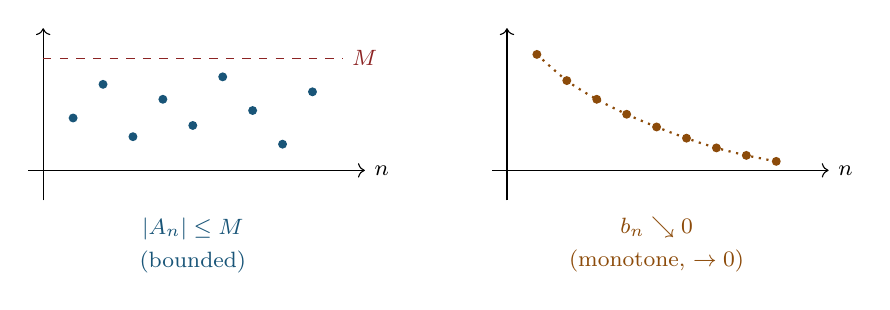
\begin{tikzpicture}[scale=0.95]
    % --- Left panel: bounded partial sums |A_n| (>= 0, capped by M) ---
    \begin{scope}
      \draw[->] (0,-0.4) -- (0,1.9);
      \draw[->] (-0.2,0) -- (4.3,0) node[right]{\footnotesize $n$};
      \draw[dashed,thmcolor] (0,1.5) -- (4,1.5) node[right]{\footnotesize $M$};
      \foreach \x/\y in {0.4/0.7,0.8/1.15,1.2/0.45,1.6/0.95,2.0/0.6,2.4/1.25,2.8/0.8,3.2/0.35,3.6/1.05}
        \fill[defcolor] (\x,\y) circle (1.7pt);
      \node[defcolor,align=center] at (2,-1.0) {\footnotesize $|A_n| \leq M$\\ \footnotesize (\alert{bounded})};
    \end{scope}
    % --- Right panel: b_n decreasing to 0 ---
    \begin{scope}[xshift=6.2cm]
      \draw[->] (0,-0.4) -- (0,1.9);
      \draw[->] (-0.2,0) -- (4.3,0) node[right]{\footnotesize $n$};
      \draw[excolor,thick,dotted] plot[smooth] coordinates
        {(0.4,1.55) (0.8,1.2) (1.2,0.95) (1.6,0.75) (2.0,0.58) (2.4,0.43) (2.8,0.3) (3.2,0.2) (3.6,0.12)};
      \foreach \x/\y in {0.4/1.55,0.8/1.2,1.2/0.95,1.6/0.75,2.0/0.58,2.4/0.43,2.8/0.3,3.2/0.2,3.6/0.12}
        \fill[excolor] (\x,\y) circle (1.7pt);
      \node[excolor,align=center] at (2,-1.0) {\footnotesize $b_n \searrow 0$\\ \footnotesize (\alert{monotone}, $\to 0$)};
    \end{scope}
  \end{tikzpicture}
  \end{center}

  \note{
    This picture shows what the two hypotheses look like. On the left, the
    blue dots are the magnitudes of the partial sums, the absolute value of
    capital "A" sub "n". Because a magnitude is never negative, the dots
    all sit above the axis, and the hypothesis says they never rise above
    the dashed red line at height capital "M". That is exactly what bounded
    means here: the sizes stay capped by capital "M", no matter how far to
    the right we go. Keep in mind that the partial sums themselves may even
    be complex numbers, which is why we track their absolute value rather
    than the sums directly. On the right, the amber dots are the values
    "b" sub "n". They
    march steadily downward toward the axis, never increasing, approaching
    zero. The whole proof lives in the tension between these two pictures:
    one factor is held in check by boundedness, the other is squeezed down
    to nothing. Let's see the strategy that combines them.
  }
\end{frame}

\begin{frame}{Proof Strategy: Theorem 3.42}
  \begin{hlbox}
  \begin{itemize}
    \item \textbf{Tool:} the partial summation formula (20).
    \item \textbf{Goal:} verify the \alert{Cauchy criterion}: make
      $\left|\sum_{n=p}^{q} a_n b_n\right|$ small for large $p$.
    \item \textbf{Key fact:} boundedness of $A_n$ plus monotonicity of $b_n$
      collapses the estimate to a \alert{multiple of $b_p$}.
  \end{itemize}
  \end{hlbox}

  \note{
    Before the formal estimate, here is the plan. The tool is the partial
    summation formula we just proved. The goal is to show the series
    satisfies the Cauchy criterion: the tail sum from index "p" to index
    "q" can be made as small as we like once "p" is large enough. The key
    fact that makes this work is the combination of two hypotheses.
    Boundedness of the partial sums capital "A" sub "n" lets us pull out a
    constant, and monotonicity of "b" sub "n" lets the differences
    telescope. Together they collapse the whole estimate down to a
    constant times "b" sub "p", which tends to zero. Let's carry it out.
  }
\end{frame}

\begin{frame}{Proof of 3.42 --- Step 1: Apply formula (20) and bound}
  \begin{proofblock}{Step 1: Insert the partial summation formula}
    Choose $M$ with $|A_n| \leq M$ for all $n$. For $N \leq p \leq q$:
    \begin{align*}
      \left|\sum_{n=p}^{q} a_n b_n\right|
        &= \left|\sum_{n=p}^{q-1} A_n(b_n - b_{n+1}) + A_q b_q - A_{p-1}b_p\right| \\
        &\leq M\left(\sum_{n=p}^{q-1}(b_n - b_{n+1}) + b_q + b_p\right).
    \end{align*}
  \end{proofblock}

  \note{
    Step one. Since the partial sums are bounded, choose a constant
    capital "M" with the absolute value of capital "A" sub "n" at most
    capital "M" for every "n". Now apply formula 20 to the tail sum and
    take absolute values. Every capital "A" appearing is bounded by
    capital "M", so we factor capital "M" out. Here is the crucial point,
    which I want you to watch on the slide: because "b" sub "n" is
    decreasing, each difference "b" sub "n" minus "b" sub "n" plus one is
    nonnegative. That is what lets us pull the absolute value inside and
    replace each term by its size without sign cancellation working
    against us. Next we evaluate that bracket.
  }
\end{frame}

\begin{frame}{Proof of 3.42 --- Step 2: Telescope and conclude}
  \begin{proofblock}{Step 2: The sum telescopes}
    The differences telescope: $\sum_{n=p}^{q-1}(b_n - b_{n+1}) = b_p - b_q$. Hence
    \[
      \left|\sum_{n=p}^{q} a_n b_n\right| \leq M\big(b_p - b_q + b_q + b_p\big) = 2M\,b_p.
    \]
    Given $\varepsilon>0$, pick $N$ with $b_N \leq \varepsilon/(2M)$. Then for $p \geq N$,
    \[
      \left|\sum_{n=p}^{q} a_n b_n\right| \leq 2M\,b_p \leq 2M\,b_N \leq \varepsilon.
    \]
    By the Cauchy criterion, $\sum a_n b_n$ \alert{converges}. \hfill$\blacksquare$
  \end{proofblock}

  \note{
    Step two finishes the argument. The sum of the consecutive differences
    telescopes: almost everything cancels, leaving just "b" sub "p" minus
    "b" sub "q". Adding the two leftover boundary terms, "b" sub "q" and
    "b" sub "p", the "b" sub "q" pieces cancel and we are left with twice
    capital "M" times "b" sub "p". This is the collapse we predicted. Now
    we use that "b" sub "n" tends to zero. Given any positive epsilon,
    choose an index capital "N" so that "b" sub capital "N" is at most
    epsilon over twice capital "M". Then for every "p" beyond capital "N",
    the tail sum is at most epsilon. That is precisely the Cauchy
    criterion, so the series converges. Let's apply this to alternating
    series.
  }
\end{frame}
}

{
\usebackgroundtemplate{%
  
\includegraphics[width=\paperwidth,height=\paperheight,keepaspectratio=false]{chapter_03_bg_04.png}%
}
% =============================================================================
\section{Alternating Series}
% =============================================================================

\begin{frame}{Theorem 3.43: Alternating Series Test}
  \begin{thmblock}{Theorem 3.43 (Leibniz)}
    Suppose
    \begin{enumerate}
      \item[(a)] $|c_1| \geq |c_2| \geq |c_3| \geq \cdots$;
      \item[(b)] $c_{2m-1} \geq 0$, $\;c_{2m} \leq 0$ \quad $(m = 1,2,3,\dots)$;
      \item[(c)] $\displaystyle \lim_{n\to\infty} c_n = 0$.
    \end{enumerate}
    Then $\sum c_n$ converges.
  \end{thmblock}

  \begin{remblock}{Terminology}
    Series satisfying (b) --- signs $+,-,+,-,\dots$ --- are \alert{alternating series}.
  \end{remblock}

  \note{
    Now a famous special case. Condition (a) says the absolute values of
    the terms are decreasing. Condition (b) says the signs alternate: the
    odd terms are nonnegative, the even terms are nonpositive, so the
    pattern of signs is plus, minus, plus, minus, and so on. Condition (c)
    says the terms tend to zero. Whenever these hold, the series converges.
    As the remark notes, series with this alternating sign pattern are
    called alternating series, and this convergence result was already
    known to Leibniz. The standard example is one minus one half plus one
    third minus one fourth and so on, the alternating harmonic series.
    First, let's build some intuition for why it converges.
  }
\end{frame}

\begin{frame}[c]{Alternating Series: Why It Converges}
  \begin{center}
  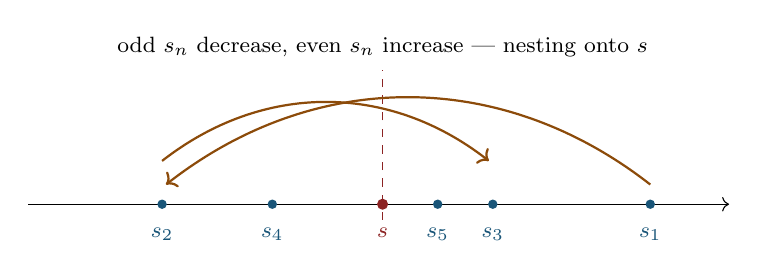
\begin{tikzpicture}[scale=1.0]
    \draw[->] (-0.3,0) -- (8.6,0);
    % limit S
    \draw[thmcolor,dashed] (4.2,-0.2) -- (4.2,1.7);
    \fill[thmcolor] (4.2,0) circle (2pt) node[below=5pt]{\footnotesize $s$};
    % partial sums
    \foreach \x/\lab/\pos in {7.6/{$s_1$}/below, 1.4/{$s_2$}/below, 5.6/{$s_3$}/below, 2.8/{$s_4$}/below, 4.9/{$s_5$}/below}
      \fill[defcolor] (\x,0) circle (1.7pt) node[\pos=5pt]{\footnotesize \lab};
    % arcs: shrinking jumps
    \draw[->,excolor,thick] (7.6,0.25) to[bend right=38] (1.45,0.25);
    \draw[->,excolor,thick] (1.4,0.55) to[bend left=38] (5.55,0.55);
    \node[align=center] at (4.2,2.0) {\footnotesize odd $s_n$ decrease, even $s_n$ increase --- \alert{nesting onto $s$}};
  \end{tikzpicture}
  \end{center}

  \note{
    Here is the geometry behind the alternating series test. Because the
    terms add and subtract in turn, each partial sum lands on the opposite
    side of the previous one. On the slide, "s" sub one sits far to the
    right; then "s" sub two jumps to the left; "s" sub three jumps back to
    the right, but not as far; and so on. Since the terms shrink in size,
    every jump is shorter than the one before, shown by the arcs getting
    smaller. The odd numbered partial sums come down from the right while
    the even numbered ones climb from the left, and they close in on each
    other like a tightening bracket. The single point they trap, marked
    "s" in red, is the sum of the series. This nesting is exactly why
    convergence is forced. Now let's see how Dirichlet's test makes it
    rigorous in a single line.
  }
\end{frame}

\begin{frame}{Proof of 3.43 --- A Corollary of Dirichlet}
  \begin{proofblock}{Proof: apply Theorem 3.42}
    Set $a_n = (-1)^{n+1}$ and $b_n = |c_n|$. Then $c_n = a_n b_n$.
    \vspace{0.4em}
    \begin{itemize}
      \item Partial sums of $a_n$: $A_n \in \{0,1\}$ --- \alert{bounded}. \checkmark\,(a)
      \item $b_n = |c_n|$ is \alert{decreasing}. \checkmark\,(b)
      \item $b_n = |c_n| \to 0$. \checkmark\,(c)
    \end{itemize}
    Hypotheses of 3.42 hold, so $\sum c_n = \sum a_n b_n$ converges. \hfill$\blacksquare$
  \end{proofblock}

  \note{
    The proof is a one-line application of Dirichlet's test, and it shows
    the power of having the general tool. We factor each term "c" sub "n"
    into a sign part and a size part. Let "a" sub "n" be minus one to the
    "n" plus one, which is plus one, minus one, plus one, and so on, and
    let "b" sub "n" be the absolute value of "c" sub "n". Then "a" sub "n"
    times "b" sub "n" reproduces "c" sub "n", signs and all. Now check the
    three hypotheses of Theorem 3.42. The partial sums of the alternating
    plus and minus ones are always either zero or one, hence bounded. The
    sizes "b" sub "n" are decreasing by assumption (a), and they tend to
    zero by assumption (c). All three conditions hold, so Dirichlet's test
    gives convergence at once. Let's turn to power series.
  }
\end{frame}
}

{
\usebackgroundtemplate{%
  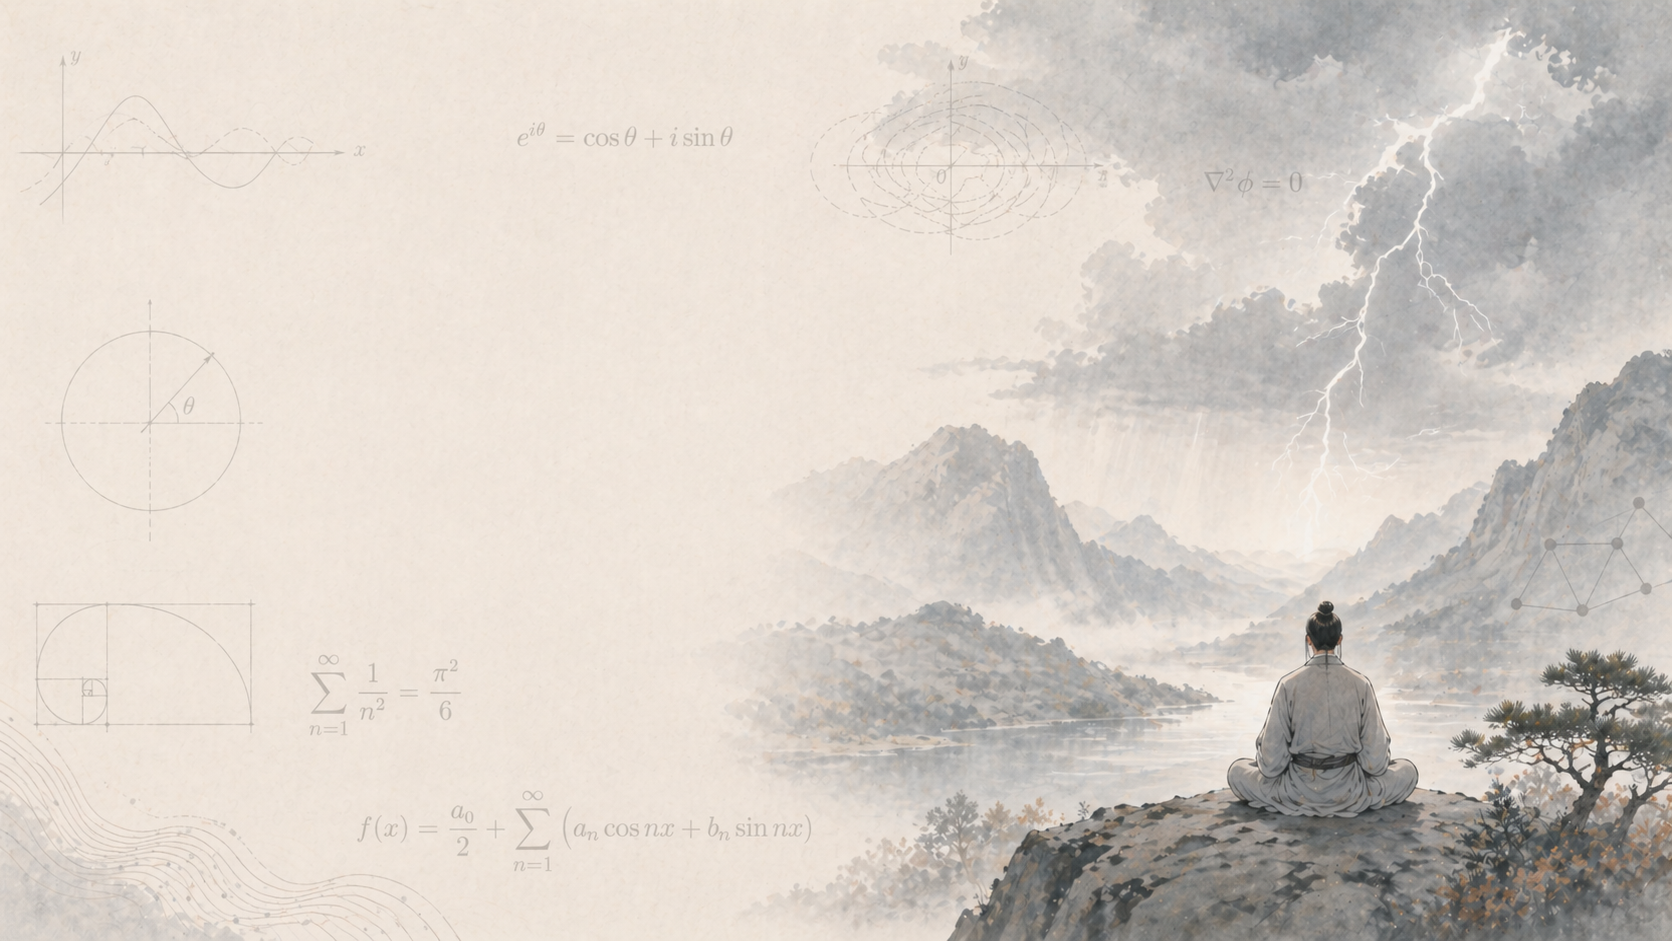
\includegraphics[width=\paperwidth,height=\paperheight,keepaspectratio=false]{chapter_03_bg_05.png}%
}
% =============================================================================
\section{Power Series on the Boundary}
% =============================================================================

\begin{frame}{Theorem 3.44: Convergence on the Unit Circle}
  \begin{thmblock}{Theorem 3.44}
    Suppose $\sum c_n z^n$ has radius of convergence $1$, and
    \[
      c_0 \geq c_1 \geq c_2 \geq \cdots, \qquad \lim_{n\to\infty} c_n = 0.
    \]
    Then $\sum c_n z^n$ converges at \alert{every} point on the circle
    $|z| = 1$, \alert{except possibly} at $z = 1$.
  \end{thmblock}

  \note{
    Our last application reaches into the complex plane. Recall from the
    previous section that a power series with radius of convergence one
    converges inside the unit disk and diverges outside it; the behavior
    right on the boundary circle, where the absolute value of "z" equals
    one, is usually subtle and was left open. This theorem settles it under
    extra hypotheses: if the real coefficients "c" sub "n" decrease to
    zero, then the series converges at every point on the boundary circle,
    with the single possible exception of the point "z" equals one. The
    point "z" equals one really can fail; think of the coefficients one
    over "n", which give the harmonic series there. Let's picture what
    this says.
  }
\end{frame}

\begin{frame}{Theorem 3.44: The Picture on the Unit Circle}
  \begin{center}
  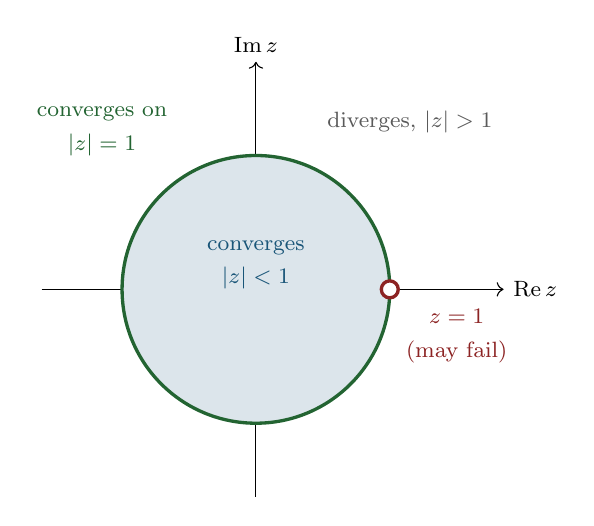
\begin{tikzpicture}[scale=1.7]
    % axes
    \draw[->] (-1.6,0) -- (1.85,0) node[right]{\footnotesize $\operatorname{Re} z$};
    \draw[->] (0,-1.55) -- (0,1.7) node[above]{\footnotesize $\operatorname{Im} z$};
    % disk interior
    \fill[defcolor!15] (0,0) circle (1);
    % boundary circle
    \draw[proofcolor,very thick] (0,0) circle (1);
    % labels
    \node[defcolor,align=center] at (0,0.18) {\footnotesize converges\\ \footnotesize $|z|<1$};
    \node[proofcolor,align=center] at (-1.15,1.18) {\footnotesize converges on\\ \footnotesize $|z|=1$};
    \node[remcolor] at (1.15,1.25) {\footnotesize diverges, $|z|>1$};
    % excluded point z = 1
    \draw[thmcolor,fill=white,very thick] (1,0) circle (1.8pt);
    \node[thmcolor,align=center] at (1.5,-0.35) {\footnotesize $z=1$\\ \footnotesize (\alert{may fail})};
  \end{tikzpicture}
  \end{center}

  \note{
    This picture summarizes the theorem in the complex plane. The shaded
    blue disk is the interior, where the absolute value of "z" is less
    than one; there the power series converges, as we already knew from
    the previous section. Outside the disk it diverges. The new content is
    the thick green boundary circle, where the absolute value of "z"
    equals one. The theorem says the series converges all the way around
    that circle, with one exception: the point "z" equals one, drawn as
    the open red dot on the right. There the series may fail, and the
    proof will show exactly why this single point is special. Let's prove
    it.
  }
\end{frame}

\begin{frame}{Proof of 3.44 --- Bounding the Geometric Partial Sums}
  \begin{proofblock}{Proof: apply Theorem 3.42 with $a_n = z^n$}
    Put $a_n = z^n$, $b_n = c_n$. For $|z|=1$, $z \neq 1$:
    \[
      |A_n| = \left|\sum_{m=0}^{n} z^m\right| = \left|\frac{1 - z^{n+1}}{1 - z}\right| \leq \frac{2}{|1-z|}.
    \]
    So $\{A_n\}$ is \alert{bounded}, while $b_n = c_n$ decreases to $0$.\\
    By Theorem 3.42, $\sum c_n z^n$ converges. \hfill$\blacksquare$
  \end{proofblock}

  \note{
    Once more, Dirichlet's test does the work. We take "a" sub "n" to be
    "z" to the "n" and "b" sub "n" to be the coefficient "c" sub "n". The
    partial sums capital "A" sub "n" are then partial sums of a geometric
    series, which we can evaluate in closed form: one minus "z" to the "n"
    plus one, all over one minus "z". When the absolute value of "z" is
    one, the numerator has absolute value at most two, so the whole
    expression is bounded by two over the absolute value of one minus "z".
    This is a fixed bound, independent of "n", as long as "z" is not equal
    to one. So the partial sums are bounded. The coefficients "c" sub "n"
    decrease to zero by hypothesis. Both conditions of Dirichlet's test
    hold, and convergence follows. Notice exactly where "z" equals one is
    excluded: there the denominator one minus "z" vanishes and our bound
    blows up. Let's summarize.
  }
\end{frame}
}

{
\usebackgroundtemplate{%
  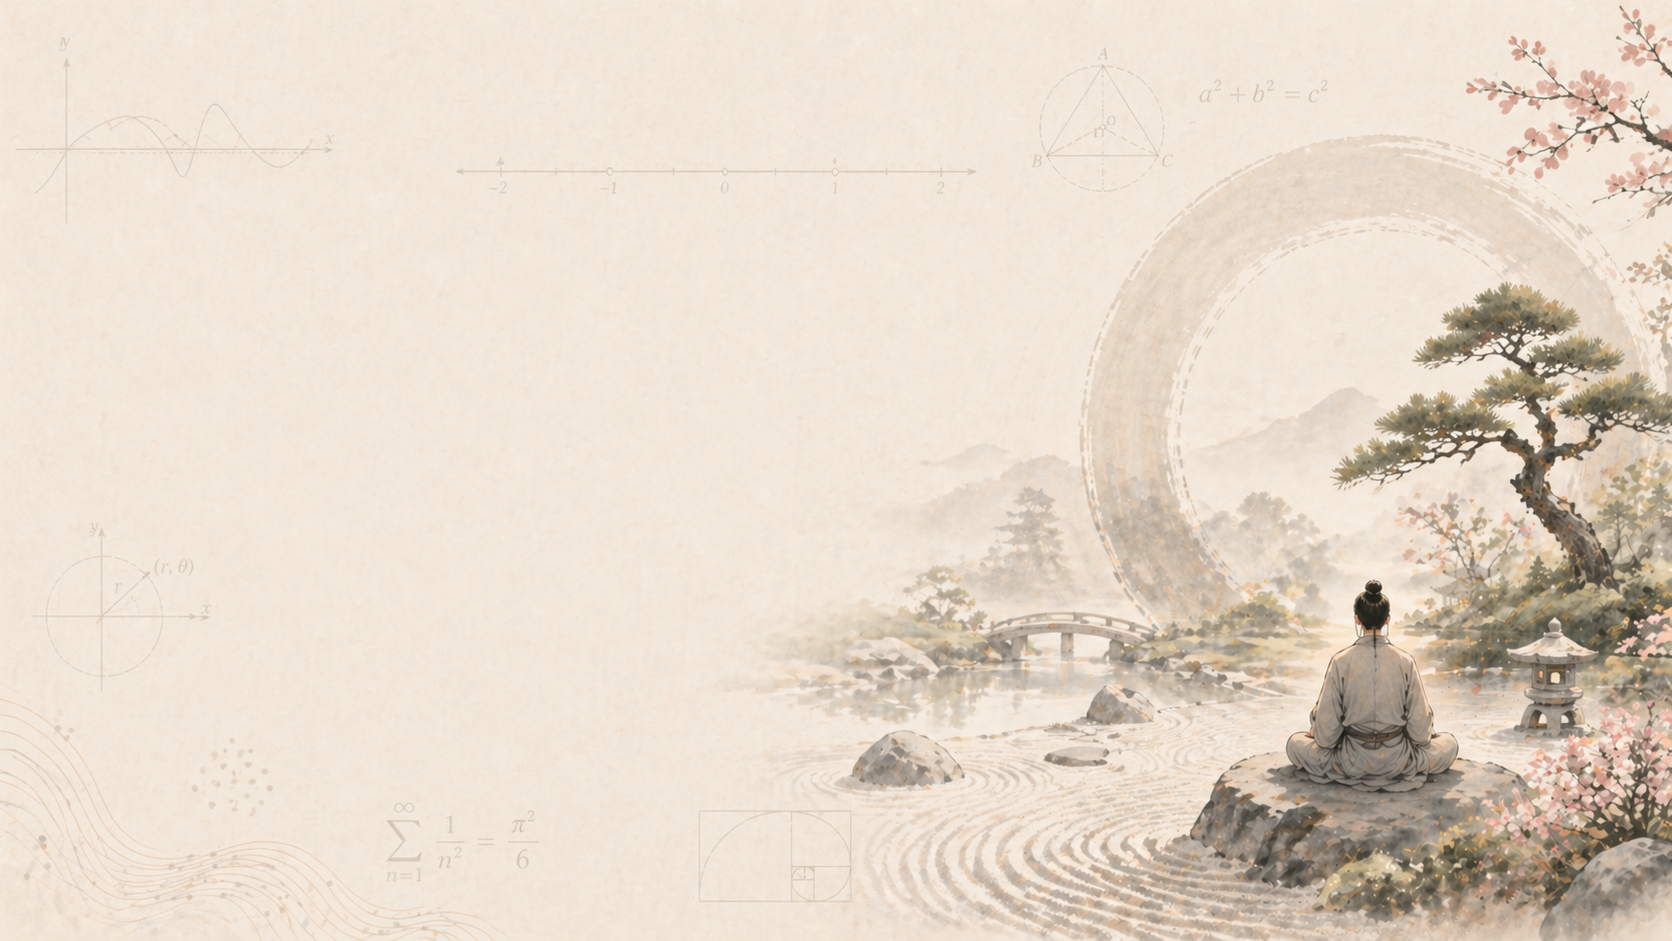
\includegraphics[width=\paperwidth,height=\paperheight,keepaspectratio=false]{chapter_03_bg_06.png}%
}
% =============================================================================
\section{Summary}
% =============================================================================

% --- Build 1/4 ---
\begin{frame}{Summary}
  \begin{hlbox}
  \textbf{Key takeaways from this section:}
  \begin{itemize}
    \item \alert{Partial summation (3.41):} the discrete integration by parts,
      \[
        \sum_{n=p}^{q} a_n b_n = \sum_{n=p}^{q-1} A_n(b_n - b_{n+1}) + A_q b_q - A_{p-1}b_p.
      \]
  \end{itemize}
  \end{hlbox}

  \note{
    Let's review what we covered. The foundation of the whole section is
    the partial summation formula, Theorem 3.41. It is the discrete
    version of integration by parts: it rewrites a sum of products "a"
    sub "n" times "b" sub "n" in terms of the partial sums capital "A"
    sub "n" and the differences of "b". This one identity powered
    everything that followed. Next, the main application.
  }
\end{frame}

% --- Build 2/4 ---
\begin{frame}{Summary}
  \begin{hlbox}
  \textbf{Key takeaways from this section:}
  \begin{itemize}
    \item \alert{Partial summation (3.41):} the discrete integration by parts.
    \item \alert{Dirichlet's test (3.42):} if $A_n$ bounded and $b_n \searrow 0$,
      then $\sum a_n b_n$ converges.
  \end{itemize}
  \end{hlbox}

  \note{
    The central application is Dirichlet's test, Theorem 3.42. It says
    that if the partial sums of "a" sub "n" stay bounded, and the second
    factor "b" sub "n" decreases monotonically to zero, then the series of
    products converges, even when it does not converge absolutely. This is
    a genuinely new kind of convergence test, complementing the root and
    ratio tests. Next, its two consequences.
  }
\end{frame}

% --- Build 3/4 ---
\begin{frame}{Summary}
  \begin{hlbox}
  \textbf{Key takeaways from this section:}
  \begin{itemize}
    \item \alert{Partial summation (3.41):} the discrete integration by parts.
    \item \alert{Dirichlet's test (3.42):} if $A_n$ bounded and $b_n \searrow 0$,
      then $\sum a_n b_n$ converges.
    \item \alert{Alternating series (3.43):} decreasing $|c_n|\to 0$ with
      alternating signs $\Rightarrow$ $\sum c_n$ converges.
  \end{itemize}
  \end{hlbox}

  \note{
    From Dirichlet's test we obtained the alternating series test, Theorem
    3.43, known already to Leibniz. If the terms alternate in sign and
    their absolute values decrease to zero, the series converges. We
    proved it in a single line by factoring out the alternating sign and
    applying Dirichlet. Next, the complex-variable consequence.
  }
\end{frame}

% --- Build 4/4 ---
\begin{frame}{Summary}
  \begin{hlbox}
  \textbf{Key takeaways from this section:}
  \begin{itemize}
    \item \alert{Partial summation (3.41):} the discrete integration by parts.
    \item \alert{Dirichlet's test (3.42):} if $A_n$ bounded and $b_n \searrow 0$,
      then $\sum a_n b_n$ converges.
    \item \alert{Alternating series (3.43):} decreasing $|c_n|\to 0$ with
      alternating signs $\Rightarrow$ $\sum c_n$ converges.
    \item \alert{Power series (3.44):} $c_n \searrow 0 \Rightarrow \sum c_n z^n$
      converges on $|z|=1$, except possibly at $z=1$.
  \end{itemize}

  \vspace{0.3em}
  \textbf{Coming up next:} Absolute Convergence.
  \end{hlbox}

  \note{
    Finally, Theorem 3.44 applied the same idea on the boundary of a power
    series disk: if the coefficients decrease to zero, the series converges
    everywhere on the unit circle except possibly at "z" equals one, where
    the geometric partial sums are no longer bounded. The lesson of the
    whole section is that one clever algebraic identity, summation by
    parts, unlocks a whole family of delicate convergence results. In the
    next section we turn to absolute convergence, and study how it differs
    from the conditional convergence we have been exploiting here. See you
    there.
  }
\end{frame}
}

\end{document}
